\documentclass[aspectratio=169,10pt]{beamer}
\usetheme{default}
\usecolortheme{seahorse}
\setbeamertemplate{navigation symbols}{}
\setbeamertemplate{footline}[frame number]
\usepackage{graphicx, booktabs, siunitx}
\graphicspath{{../figures/}}

\title{SiPM-Wall Bars: Top/Bottom Combination \& Vertical Position}
\subtitle{n\_TOF EAR2 X17 --- run 224404, wall--plastic MIP coincidences}
\author{Dylan Neff \\[0.5ex] {\small analysis and slides prepared with Claude (Anthropic AI assistant)}}
\date{July 17, 2026}

\begin{document}

\begin{frame}\titlepage\end{frame}

\begin{frame}{Setup: what the two ends give us}
\begin{columns}
\column{.54\textwidth}
\begin{itemize}
\item Wall bars are \textbf{vertical}, $\sim$50 cm, read by \textbf{top} and
      \textbf{bottom} SiPMs (detn odd/even; 4 groups of 4 bars per arm).
\item Two ends of the same deposit $\Rightarrow$ three things to try:
\begin{enumerate}
  \item combine amplitudes for a position-independent MIP estimate
        (geometric vs arithmetic mean);
  \item vertical position from amplitude asymmetry $\ln(A_{\rm top}/A_{\rm bot})$;
  \item vertical position from timing $t_{\rm bot}-t_{\rm top}$.
\end{enumerate}
\item Same clean MIP sample as before: same-arm wall$\times$plastic coincidence,
      late tof, sideband-subtracted ($16/100$).
\end{itemize}
\column{.46\textwidth}
\centering
$A_{\rm top}=A_0\,e^{-(L/2-y)/\lambda}$\\
$A_{\rm bot}=A_0\,e^{-(L/2+y)/\lambda}$\\[1ex]
\rule{.8\textwidth}{0.4pt}\\[1ex]
$\sqrt{A_{\rm top}A_{\rm bot}}=A_0e^{-L/2\lambda}$ \; (no $y$)\\[0.6ex]
$\ln\!\frac{A_{\rm top}}{A_{\rm bot}}=\frac{2y}{\lambda}$,\quad
$t_{\rm bot}-t_{\rm top}=\frac{2y}{v_{\rm eff}}$
\end{columns}
\end{frame}

\begin{frame}{(2) Combine the ends: geometric mean is (slightly) best}
\centering
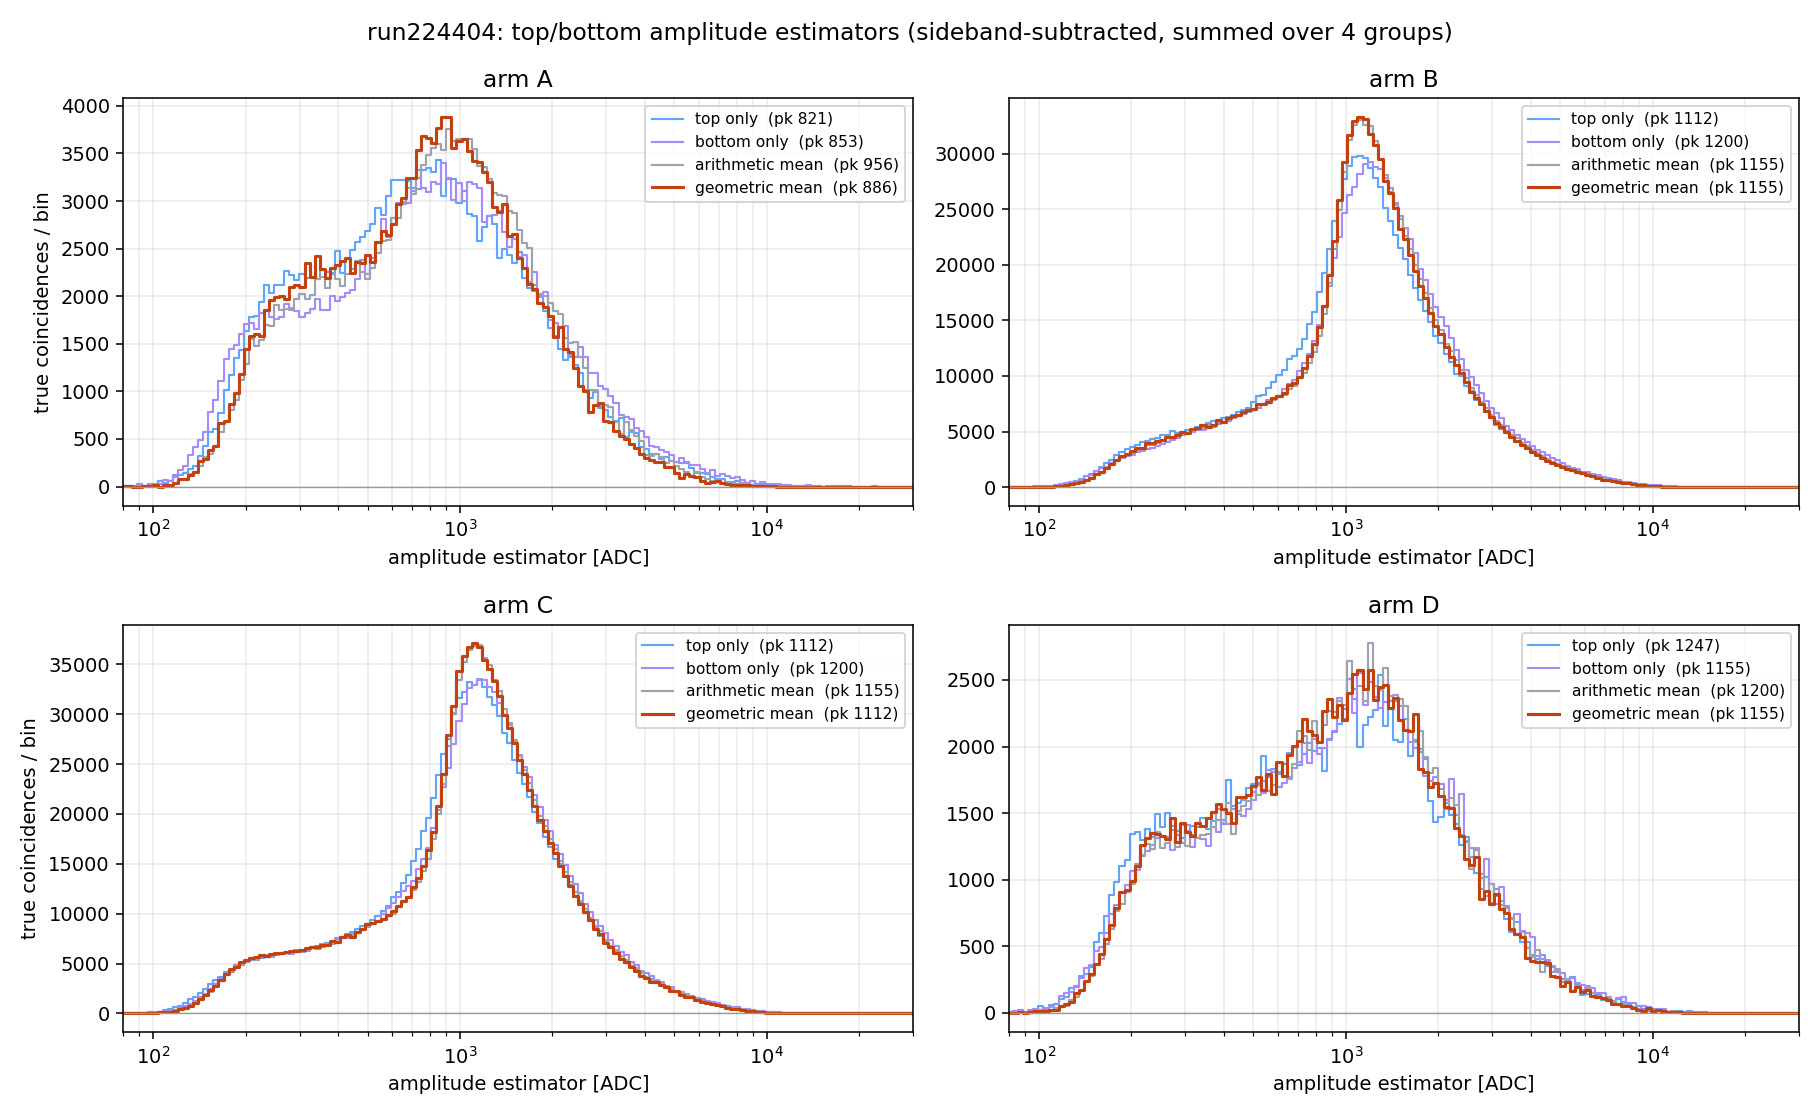
\includegraphics[height=.66\textheight]{16_vertical/estimator_comparison.png}\\
{\footnotesize B/C: geometric mean gives the sharpest MIP peak (FWHM/peak
$\approx0.90$--$0.96$ vs $1.0$--$1.1$ single-ended); arithmetic mean nearly ties it.
The two means agree because attenuation is \emph{weak} ($\lambda\!\gg\!L$, next slides).
A/D: no MIP peak (accidental-dominated).}
\end{frame}

\begin{frame}{Why geo $\approx$ arith here: $A_{\rm top}$ vs $A_{\rm bot}$}
\begin{columns}
\column{.55\textwidth}
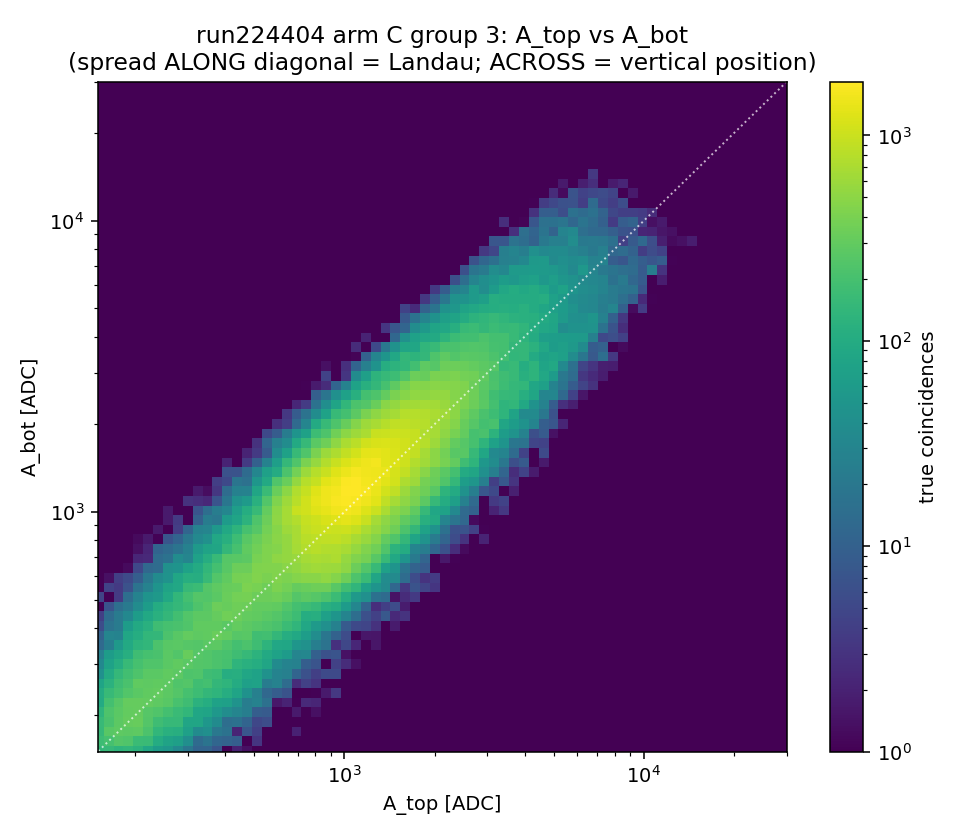
\includegraphics[width=\textwidth]{16_vertical/attenuation_C_g3.png}
\column{.45\textwidth}
\begin{itemize}
\item Spread \textbf{along} the diagonal = the (large) Landau energy fluctuation,
      \emph{correlated} between the two ends.
\item Spread \textbf{across} the diagonal = vertical position (attenuation
      asymmetry) --- much smaller.
\item Geometric mean projects along the diagonal $\Rightarrow$ keeps the energy,
      cancels position. Since the across-spread is small, arithmetic mean does
      almost as well.
\end{itemize}
\end{columns}
\end{frame}

\begin{frame}{(1) Split by plastic bar: MIP peak is bar-independent}
\centering
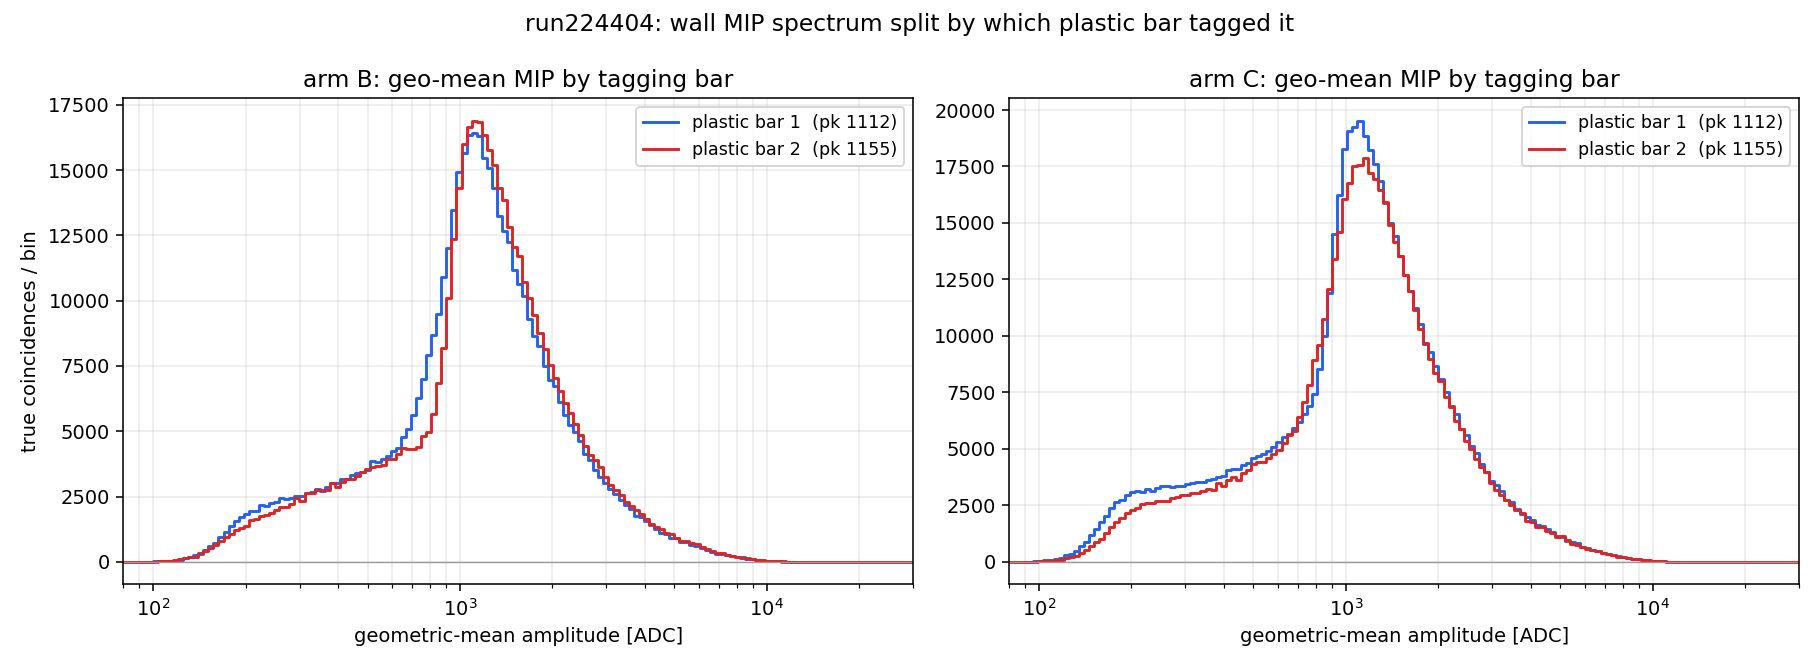
\includegraphics[height=.66\textheight]{16_vertical/geo_by_bar.png}\\
{\footnotesize Wall geo-mean MIP spectrum split by which plastic bar tagged the
coincidence. Peaks agree to one bin (1112 vs 1155 ADC) on both arms
$\Rightarrow$ merging the two bars (as the main analysis does) is safe; the low-amp
shoulders differ, tracking the bar$\leftrightarrow$u-half geometry.}
\end{frame}

\begin{frame}{(3) Vertical position: amplitude and timing both work}
\centering
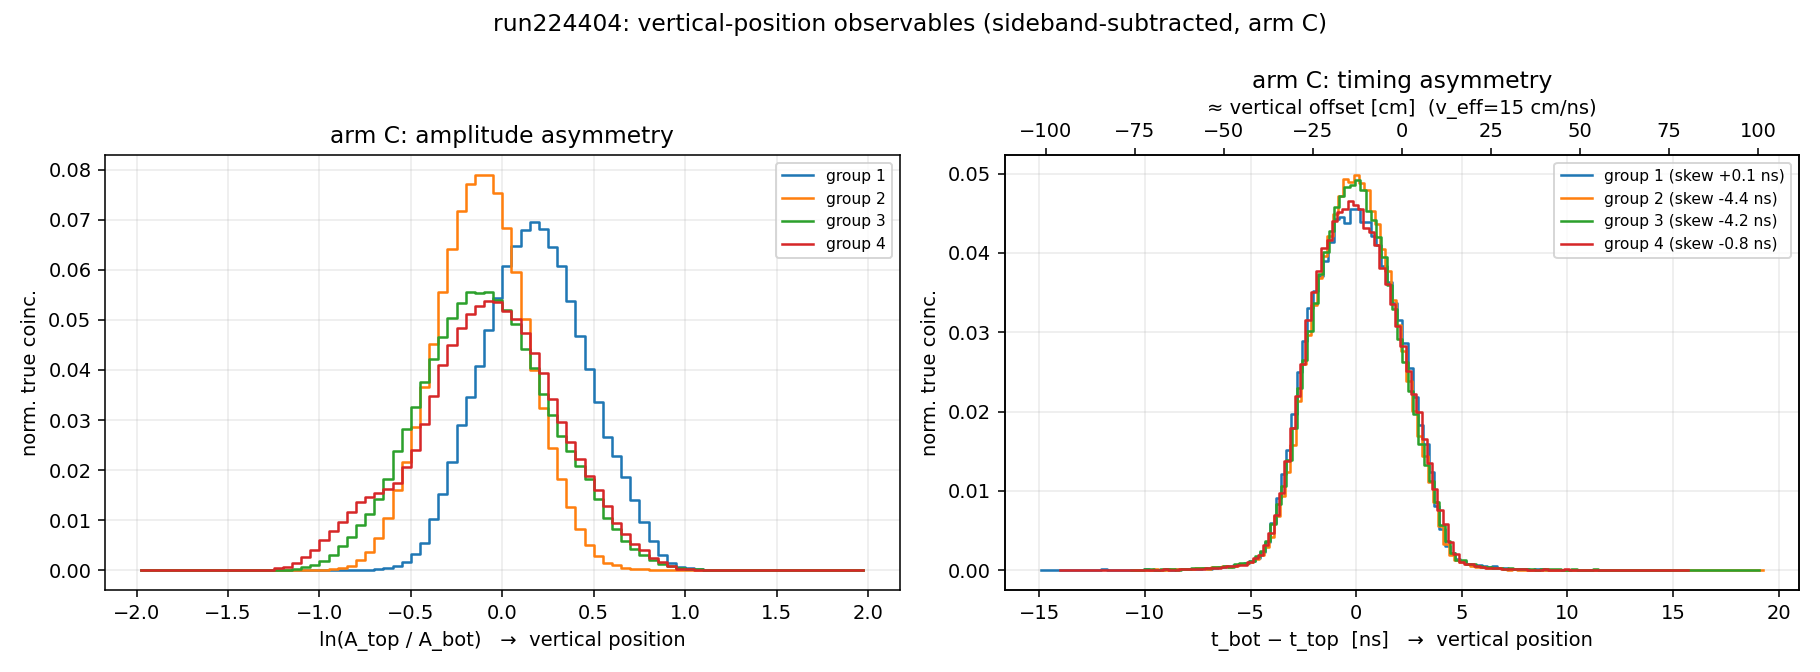
\includegraphics[width=.98\textwidth]{16_vertical/position_1d_C.png}\\
{\footnotesize Sideband-subtracted, per group (arm C). Both $\ln(A_{\rm top}/A_{\rm bot})$
and the cable-skew-corrected $t_{\rm bot}-t_{\rm top}$ span the bar; the top axis
converts timing to cm ($v_{\rm eff}=15$ cm/ns).}
\end{frame}

\begin{frame}{The two estimators agree $\Rightarrow$ real vertical coordinate}
\begin{columns}
\column{.58\textwidth}
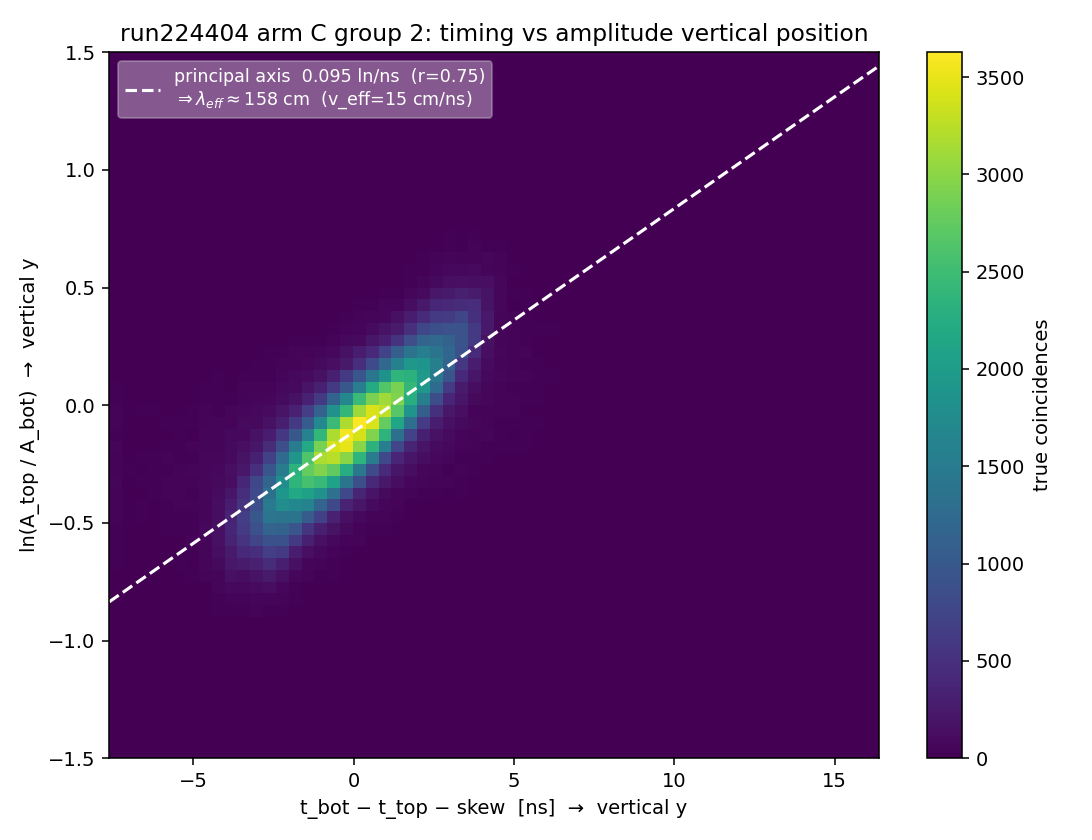
\includegraphics[width=\textwidth]{16_vertical/position_corr_C_g2.png}
\column{.42\textwidth}
\begin{itemize}\footnotesize
\item Tight correlation ridge ($r\approx0.75$): timing and amplitude track the
      \emph{same} vertical $y$.
\item Slope $=v_{\rm eff}/\lambda_{\rm eff}\Rightarrow
      \lambda_{\rm eff}\approx100$--$160$ cm (consistent across all 8 B/C groups)
      --- i.e.\ $\sim$2--3$\times$ the bar length, hence weak attenuation.
\item Single-hit vertical resolution $\sigma_y\approx$ \textbf{10--13 cm} from
      \emph{either} method ($\sim$4--5 elements over 50 cm); combining them is
      tighter still.
\end{itemize}
\end{columns}
\end{frame}

\begin{frame}{Summary}
\begin{itemize}
\item \textbf{Plastic bars:} plotting the wall MIP spectrum separately per tagging
      bar gives the \emph{same} peak $\Rightarrow$ the standard bar-merged spectrum
      is unbiased.
\item \textbf{Top/bottom amplitude:} use the \textbf{geometric mean}
      $\sqrt{A_{\rm top}A_{\rm bot}}$ --- sharpest, position-independent MIP peak;
      arithmetic mean is a close second because $\lambda_{\rm eff}\gg L$.
\item \textbf{Vertical position is recoverable}, and cross-validated two ways:
      amplitude asymmetry and top/bottom timing agree ($r\approx0.75$), both giving
      $\sigma_y\approx10$--$13$ cm over the 50 cm bar.
\item Byproduct: $\lambda_{\rm eff}\approx100$--$160$ cm and $v_{\rm eff}\approx15$
      cm/ns effective --- can be pinned exactly with a triggered/known-position
      sample.
\item Caveat: 4 bars are ganged per group $\Rightarrow$ this is a per-group vertical
      $y$, with the horizontal (u) coordinate only at group / plastic-bar granularity.
\end{itemize}
\end{frame}

\end{document}
